
\begin{wrapfigure}{r}{0.4\textwidth}
  \begin{center}
    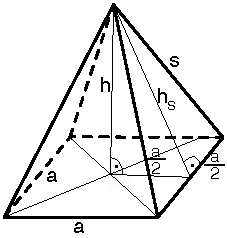
\includegraphics[width=0.38\textwidth]{pyramid_fig}
  \end{center}
  \caption{Pyramide}
\end{wrapfigure}

\Aufgabe{Pyramide-Kantenlänge (10 Punkte)}
  
 Schreiben Sie Prozeduren, die die Kantenlänge einer
  Pyramide berechnen!  Von der Pyramide ist die Seitenlänge der
  Grundfläche $a$ und die Höhe $h$ gegeben.

  Die Kantenlänge einer Pyramide ist die Summe der Kantenlänge der
  quadratischen Grundfläche (mit Seitenlänge $a$) und der Länge der
  vier nach oben gehenden Kanten $s$.  Schreiben Sie Prozeduren, die
  folgende Teilprobleme lösen:



  \begin{enumerate}
  \item Schreiben Sie eine Prozedur \texttt{square-circumference}, die
    den Umfang der quadratischen Grundfl\"ache berechnet.

 \item Um $h_s$ und $s$ zu berechnen, brauchen Sie jeweils den
    \textit{Satz des Pythagoras}: $ a^2 + b^2 = c^2$\\
    Schreiben Sie eine Prozedur \texttt{pythagoras}, die das $c$ der
    obigen Gleichung berechnet.  Erkennen und abstrahieren Sie weitere
    Teilprobleme!

  \item Schreiben Sie eine Prozedur \texttt{pyramid-one-edge-length}, die
    die Länge $s$ berechnet (dazu brauchen Sie die Länge $h_s$).

  \item Schreiben Sie schließlich eine Prozedur
    \texttt{pyramid-edge-length}, die die Kantenlänge der Pyramide
    berechnet.  Benutzen Sie dafür die bisher geschriebenen
    Prozeduren. 
  \end{enumerate}

  \textbf{Hinweis:} Zur Lösung können Sie die eingebaute Scheme-Prozedur
    \texttt{sqrt}, die die Signatur \texttt{(number -> number)} besitzt,
    verwenden: \texttt{(sqrt x)} liefert die Quadratwurzel von $x$.\\

Abgabe: 
    Programm \texttt{pyramid-edge.rkt}


  \begin{solution}
     \smallskip
    Punkteverteilung:
    \begin{itemize}
    \item 4 Punkte Kurzbeschreibungen, Vertr"age \& Testf"alle
    \item 1 Punkt Ger\"ust \& Rumpf \texttt{square-circumference}
    \item 2 Punkte Ger"ust \& Rumpf \texttt{pythagoras}
    \item 2 Punkte Ger"ust \& Rumpf \texttt{pyramid-one-edge-length} 
    \item 1 Punkt Ger\"ust \& Rumpf \texttt{pyramid-edge-length}
    \end{itemize}

\pagebreak
\lstinputlisting[caption=Pyramidenproblem - Lösung]{pyramid-edge.rkt}     
  \end{solution}

